% !TeX root = ../../../book.tex
\subsection{求和杂谈}\label{sec:section1.4.3}

\subsubsection*{奇数求和:观察模式}

既然谈到了整数求和,不妨探讨一些相关问题。首先介绍一种有趣的几何方法来解释奇数之和:将 $1$ 表示为 $1 \times 1$ 方块,随后每个连续的更大奇数可视作由 $1 \times 1$ 方块构成的直角,它能完美贴合前一个图形。我们为什么要这样做?因为奇数序列中连续项相差 $2$,每次将直角边增加 $1$ 个方块,即可与原图形无缝衔接,逐步构建更大的正方形!

\begin{center}
    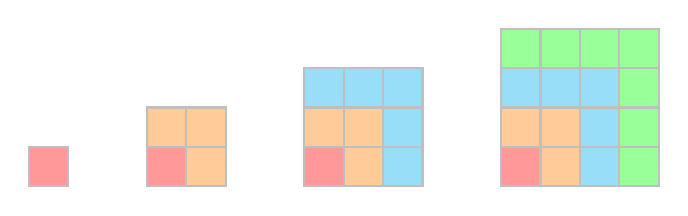
\begin{tikzpicture}[thick,scale=0.5, x=1cm, y=1cm]
        \foreach \x in {0,3,7,12}
        {
            \fill[red!40!white] (\x, 0) rectangle ++ (1,1);
            \draw[lightgray] (\x, 0) rectangle ++ (1,1);
        }

        \foreach \x in {3,7,12}
        {
            \foreach \i in {0,1}
            {
                \fill[orange!40!white] (\x+\i, 1) rectangle ++ (1,1);
                \draw[lightgray] (\x+\i, 1) rectangle ++ (1,1);
                \fill[orange!40!white] (\x+1, \i) rectangle ++ (1,1);
                \draw[lightgray] (\x+1, \i) rectangle ++ (1,1);
            }
        }

        \foreach \x in {7,12}
        {
            \foreach \i in {0,...,2}
            {
                \fill[cyan!40!white] (\x+\i, 2) rectangle ++ (1,1);
                \draw[lightgray] (\x+\i, 2) rectangle ++ (1,1);
                \fill[cyan!40!white] (\x+2, \i) rectangle ++ (1,1);
                \draw[lightgray] (\x+2, \i) rectangle ++ (1,1);
            }
        }

        \foreach \i in {0,...,3}
        {
            \fill[green!40!white] (12+\i, 3) rectangle ++ (1,1);
            \draw[lightgray] (12+\i, 3) rectangle ++ (1,1);
            \fill[green!40!white] (12+3, \i) rectangle ++ (1,1);
            \draw[lightgray] (12+3, \i) rectangle ++ (1,1);
        }
    \end{tikzpicture}
\end{center}

这种模式会持续下去吗?若确信如此,要如何严格证明?几何图案隐含的数值之和有何意义?这是首先要回答的问题,因为尽管几何呈现直观优美,但却难以精确操作和验证,最终无法给出严谨的\emph{证明}。本质上,仅展示前几项并宣称``看,它成立!''并不构成数学证明,因此需要寻求更优的表述方式。这并非否定图形的意义与美感,其运作机制确实提供了有价值的数学洞察,但归根结底,这便是其所能带给我们的上限。

\subsubsection*{奇数求和:证明我们的发现}

让我们尝试用数字形式写出上图所表示的求和。每个正方形由 $1 \times 1$ 块组成,每个比前一个多两块,因此每个正方形对应一个求和,例如
\[1 \qquad 1+3 \qquad 1+3+5 \qquad 1+3+5+7 \]
依此类推。从这些求和中,我们注意到它们都是平方数:
\[1=1^2 \qquad 1+3=4=2^2 \qquad 1+3+5=9=3^2 \qquad 1+3+5+7=16=4^2 \]
\emph{这}正是我们想要证明的模式;它对应于之前观察到的几何图形,但现在是我们可以操作的数学形式。现在,让我们思考如何证明这一点。这种模式与我们之前见过的模式相似吗?我们之前已经证明过关于整数之和的结果了吗?当然!回顾之前的题目,事实上在某些方面,我们已经证明了
\[1 + 2 + 3 + \dots + (n_1) + n =\frac{n^2 + n}{2}\]
这对该题有何用处?我们证明的求和公式涉及从 $1$ 到 $n$ 的\emph{所有}连续整数,但当前问题只考虑连续\emph{奇数}。

之前我们用函数 $S(n)$ 表示前 $n$ 个自然数之和,所以我们定义函数 $T(n)$ 表示前 $n$ 个奇数之和。首先,我们需要确定这个和的项,然后尝试将它们与 $S(n)$ 联系起来。下面,我们列出了 $n = 1, 2, 3, 4$ 时的和。你能找到一种方法来识别求和中的最大项并用 $n$ 表示它吗?
\begin{align*}
    n=1: &\quad 1\\
    n=2: &\quad 1+3\\
    n=3: &\quad 1+3+5\\
    n=4: &\quad 1+3+5+7
\end{align*}
请注意,求和项的最后一项始终为 $2n-1$。这与一般事实相关,即任何偶数都可以表示为 $2k$ 其中 $k$ 为整数,任何奇数都可以表示为 $2n - 1$,其中 $n$ 为整数。(类似地,奇数也可表示为 $2n + 1$,但这里使用 $2n - 1$ 更合适。)因此,前 $n$ 个奇数之和的公式为
\[T(n) = 1 + 3 + 5 + 7 + \dots + (2n - 3) + (2n - 1)\]
我们能否将这个求和与 $S(n)$ 或其他公式联系起来?请注意求和公式
\[S(2n) = 1 + 2 + 3 + \dots + (2n - 3) + (2n - 2) + (2n - 1) + 2n\]
包含从 $1$ 到 $2n$ 的\emph{所有}自然数,而 $T(n)$ 仅包含该范围内的奇数。或许将两个和相减,并求剩余项之和是合理的:
\begin{align*}
    S(2n) - T(n) &= 1 + 2 + 3 + \dots + (2n - 1) + 2n \\
    &\quad -\left(1 + 3 + 5 + \dots + (2n - 3) + (2n - 1)\right) \\
    & =  2 + 4 + 6 + \dots + (2n - 2) + 2n
\end{align*}
这些项都是从 $2$ 到 $2n$ 的\emph{偶数}。我们如何求得这个和?我们是否需要做额外的工作,还是可以应用之前的证明结果?由于所有项都是\emph{偶数},我们可以将所有项除以 $2$ 并写成
\begin{align*}
    \frac{1}{2}\left(S(2n) - T(n)\right) &= \frac{1}{2}\left(2 + 4 + 6 + \dots + (2n - 2) + 2n\right)\\
    &= 1 + 2 + 3 + \dots + (n - 1) + n = S(n)
\end{align*}
可以确认,最右边求和中的所有项都是整数。不仅如此,它们\emph{都是}从 $1$ 到 $n$ 的连续整数,而我们知道其求和公式!现在,所有内容都用已知公式 $S(n)$ 和 $S(2n)$ 以及所求公式 $T(n)$ 表达。最后一步是整理方程,解出 $T(n)$,并代入 $S$ 的公式:
\begin{align*}
    \frac{1}{2}\left(S(2n) - T(n)\right) &= S(n) \\
    S(2n) - T(n) &= 2S(n) \\
    T(n) &= S(2n) - 2S(n) \\
    T(n) &= \frac{(2n)^2 + 2n}{2} - \frac{2 \cdot (n^2 + n)}{2} \\
    T(n) &= \frac{4n^2 + 2n - 2n^2 - 2n}{2} \\
    T(n) &= \frac{2n^2}{2} \\ 
    T(n) &= n^2
\end{align*}
这看起来很好,不是吗?尽管需要一些代数运算,但我们得出了要证明的结论:连续奇数之和是完全平方数。不仅如此,我们还成功地精确证明了该平方数与求和项数之间的关系。具体来说,结论可简洁概括为``前 $n$ 个奇数之和等于 $n^2$''。

\subsubsection*{另一种解法:归纳证明}

我们能否用不同的方式证明这个结论?如果尚未证明上一节的结论,或者未想到那种证明方法怎么办?能否利用最初观察到的和的结构特征?

让我们换个角度思考。具体而言,探究为何在求和序列中添加一项会产生新的平方数。假设已知某个求和结果等于平方数(例如 $1 = 1^2$),现在\emph{假设}对任意项数 $n$ 均有:
\[1 + 3 + 5 + \dots + (2n - 3) + (2n - 1) = n^2\]
基于此,能否推断下一个和?添加后续奇数 $2n + 1$ 后:
\[1 + 3 + 5 + \dots + (2n - 3) + (2n - 1) + (2n + 1) = n^2 + 2n + 1 = (n + 1)^2\]
这证实了我们的推测:若前 $n$ 个奇数之和为 $n^2$,则前 $n+1$ 个奇数之和必为 $(n+1)^2$。但这是否构成完整证明?通过假设结论成立来推进证明是否合理?

这种通过已知形式推导``后续''形式的策略称为\textbf{数学归纳法}(一般来说,``后续''一词的含义取决于上下文;此处它的含义指增加求和项)。下一章将深入探讨此方法。当前需要强调的是:该策略完全有效,但高度依赖初始条件 $1 = 1^2$ 的正确性。由此可逐步推得 $1+3=2^2, 1+3+5=3^2$ 等结论。若初始条件不成立会怎样?这对归纳法有何启示?我们将在后续讨论中解决这些问题。

\subsubsection*{泛化:算术级数}

我们将探讨的最终求和问题与前两个问题密切相关。事实上,若能证明接下来的结论,就不必证明前两个结论!在这个意义上,接下来的结论更强:其真实性蕴含了前两个结论的真实性。(这是数学中常见的关系,用于描述结论之间的相对强度。)

现在,我们要为一般的\textbf{算术级数}建立一个求和公式。这意味着我们将对一个公差为固定值的级数求和,或者说,每一项由前一项加上一个固定常数得到。请注意,后两个题目中的求和对象都是算术级数:第一个求和的公差为 $1$(即每项加 $1$ 得到下一项),第二个求和的公差为 $2$(即每项加 $2$ 得到下一项)。

如何表示一个一般的算术级数?由于连续项之间相差一个固定常数,我们设此常数为 $c$。求和还需首项,设其为 $a$。此外,我们需要知道求和项数,设其为 $k$(沿用之前的变量含义)。于是,可用这三个变量表示整个求和:
\[A(a, c, k) = a + (a + c) + (a + 2c) + (a + 3c) + \dots + \left(a + (k - 2)c\right) + \left(a + (k - 1)c\right)\]
我们利用了公差为 $c$ 的性质:首项为 $a$,第二项为 $a + c$,依此类推。总项数为 $k$,首项可视为 $a + 0 \cdot c$,末项则是首项加 $k - 1$ 次 $c$ 的结果(因为从 $0$ 到 $k - 1$ 共有 $k$ 个数)。符号 $A(a, c, k)$ 表示``首项为 $a$、公差为 $c$、项数为 $k$ 的算术级数之和''。现在,如何计算这个求和?

沿用之前有效的策略:在第一个求和中,我们将级数正序与倒序相加,形成具有相同和的配对项,从而将求和转化为乘法。我们尝试将此法应用于此:
\begin{center}
    \begin{tabular}{ccccccccc}
                 a & + &      (a+c) & + & \dots & + & (a+(k-1)c) & = & A(a,c,k)\\\noalign{\smallskip\smallskip}
        (a+(k-1)c) & + & (a+(k-2)c) & + & \dots & + &          a & = & A(a,c,k)\\\noalign{\smallskip\smallskip}
        \hline
        (2a+(k-1)c)& + & (2a+(k-1)c)& + & \dots & + &(2a+(k-1)c) & = &2A(a,c,k)\\\noalign{\smallskip\smallskip}
    \end{tabular}
\end{center}
我们发现每个配对项之和均为 $2a + (k-1)c$。这样的配对项有多少?共有 $k$ 项(这正是我们选用 $k$ 的原因)。将求和表示为乘法,可得:
\[2A(a, c, k) = k \cdot (2a + (k - 1)c)\]
因此
\[A(a, c, k) = \frac{k}{2} \cdot k \cdot (2a + (k - 1)c)\]
这个结果是否符合你的预期?有时,尝试``猜测''可能的结果,再与推导结论对比,有助于理解其意义。

\subsubsection*{具体应用}

前文讨论的求和问题均为算术级数,那么该公式能否正确求解呢?第一题中取 $a = 1,c = 1, k = n$;代入公式得:
\[A(1, 1, n) = \frac{1}{2} \cdot k \cdot \left(2 + (n - 1)\right) = \frac{n}{2} \cdot(n+1) = \frac{n^2+n}{2}\]
这与我们之前的结论一致。对于第二题,变量取值如何?公式是否成立?请你自行验证结果。

\subsubsection*{另一种表示}

最后我们探讨该公式的另一种表达形式。观察括号中的项 $a + \left(a + (k-1)c\right)$,其结构是否有特殊意义?事实上,它们恰好是求和的首项与末项。因此求和公式可改写为:$A(a, c, k) = \frac{k}{2}(a + b)$,其中 $a$ 为首项,$b$ 为末项。这种形式有时更便捷。

例如求首项为 $12$、末项为 $110$、共 $14$ 项的算术级数之和,无需计算公差 $c$ 即可直接求解:$\frac{14}{2} \cdot (12 + 110) = 854$。这种方法是否更高效?此时公差 $c$ 是多少?给定 $a,b,k$ 时,是否存在快速求解 $c$ 的方法?

\subsubsection*{解题心得}

掌握已有结论有助于简化证明过程。有时虽知结论可用,却难觅应用之法。在这种情况下,我们意识到已证明的求和公式或许可以推广到其他求和,因此尝试将其应用于新问题。值得注意的是,奇数求和公式存在不依赖旧结论的独立证法。这暗示了更通用的结论——我们通过研究一般算术级数实现了这种推广。

在解决前两个求和问题时,我们采用了多种策略,但仅将其中一种策略应用于一般级数问题。这些方法能否迁移至其他场景?能否用数学归纳法证明第一个公式?能否用正序/逆序相加技术证明第二个公式?建议你尝试实践一下这些策略。这么做虽看似冗余(因为结论已知),但理解不同技术在不同情境下的应用是宝贵经验。数学证明中,策略选择往往与结论推导同等重要。因此,通过专项练习培养策略直觉,洞察其适用边界,将大有裨益。
